\documentclass{article}
\usepackage{graphicx}
\usepackage{float}

\title{Human Computer Interaction \\ Coursework 2}
\author{Shaw Eastwood, s.eastwood@rgu.ac.uk}

\begin{document}
	\maketitle

	\section{User Feedback}
	The user feedback recieved described in this section will inform the on the designs reviewed in the next section.
	A series of questions were sent out and users asked to respond on these, below are the results.
\begin{table}[H]
\hspace{-3cm}
\begin{tabular}{lllcp{3cm}llc}
\hline
	name & age & occupation & native & question1 & question2 & question3 & question4 \\
\hline
	Adam & 21 & Student & Yes & Check for transport availability & Yes & Yes & None \\
	Liam & 22 & Student & Yes & Opening times of venue & Yes & No & Have to sign up \\
	Steve & 45 & Mechanic & No & Access by public transport & No & No & Internet Acess \\
	Anne & 24 & Researcher & No & Public Transport access and opening times & No & Yes & the past locations \\
	Luke & 22 & Software Engineer & Yes & Ability to filter by distance, opening times & Yes & Yes & None \\
	James & 20 & Barista & No & Filter by cost/opening times & Yes & Yes & None \\
	Alice & 23 & Developer & No & Only see highly rated locations & Yes & Yes & None \\
	John & 31 & Carpenter & No & Link to the pages website, pictures of the place, make bookings for tours & No & Yes & Tracking of any kind \\
	Bill & 29 & IT & Yes & If the place has food onsite, if not nearby locations & Yes & Yes & None \\
\hline
\end{tabular}
\end{table}
	As observed from the results above we can see that the primary concerns are mostly in the core functionality previously discussed but the addition of a "nearby locations" would help increase the user experience.
	Conversely we can see that the decision to not include a profile function in the early prototyping was useful as some respondents raised concerns with data collection.
	However a number of the core features, such as the rating and the photo adding will require this feature.
\section{Initial Scenario Based Designs}
It is worth mentioning for all of the following designs it is expected to be be nested inside of a standard Mobile Phone UI, and thus back functionality is provided by the implementation of the users individual phone manufacturer.
\subsection{Design 1}
\section{table0}
\hspace{-1cm}
	\centering
	\begin{tabular}{p{4cm}p{10cm}}
		\hline
		Title & tourism app \\
		\hline
		Date & 16th April 2019 \\
		\hline
		Scene & 1 of 4 \\
		\hline
		Description & This is the landing page \\
		\hline
		Links From Scenes & N/A \\
		\hline
		Links To Scenes & Scene 2 \\
		\hline
		\multicolumn{2}{c}{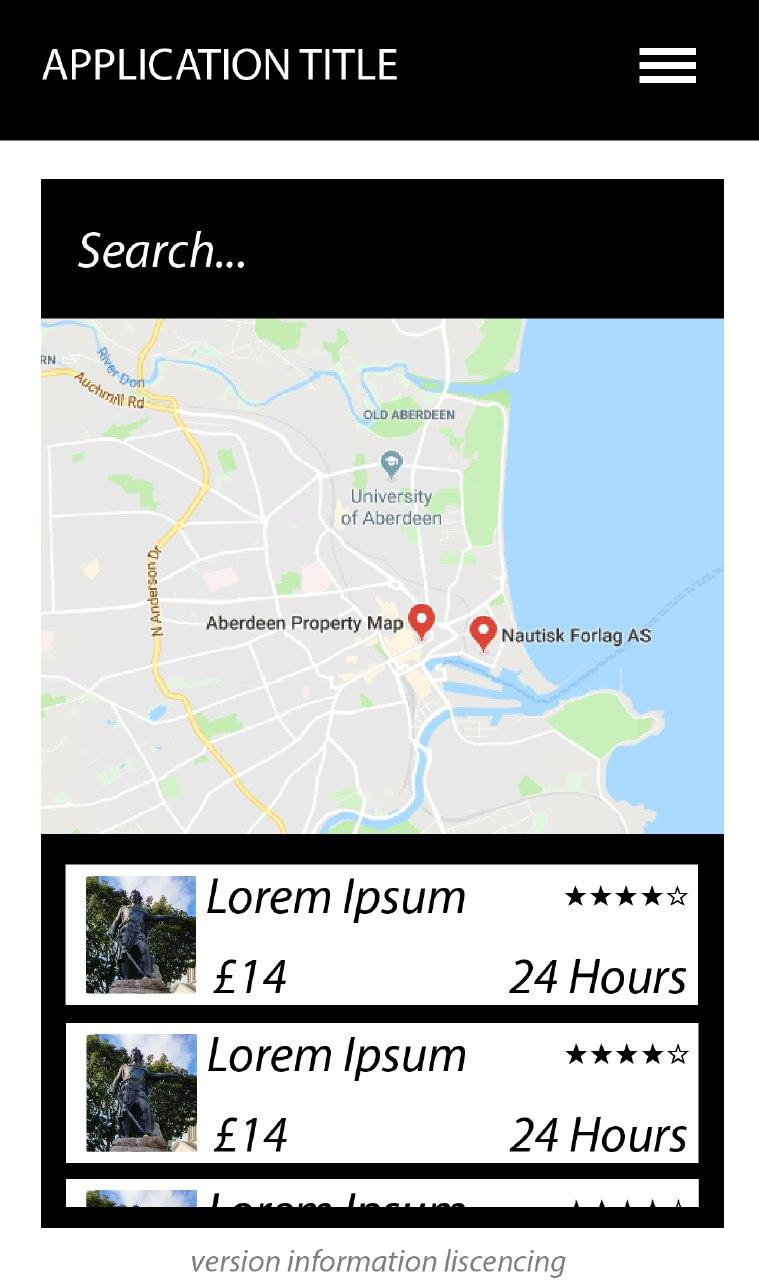
\includegraphics[width=0.5\linewidth]{images/screen0.jpg}} \\
		\hline
		Background & Standard phone background \\
		\hline
		Colour Scehemes Used & Default to black and white but would import from the system theme so users feel immersed \\
		\hline
		Text Attributes & Again, follows system theme (usually a sans-serif font). \\
		\hline
		Audio Files & N/A \\
		\hline
		Video Files & N/A \\
		\hline
		Stills Files & N/A \\
		\hline
		Animations / Movie Clips & N/A \\
		\hline
		\multicolumn{2}{c}{Interface Components (buttons, widgets)} \\
		\hline
		\multicolumn{2}{p{14cm}}{The interface consists of a number of bold, large buttons for the user to choosefrom linking to the various, primary, function of the app} \\
		\hline
	\end{tabular}

\hspace{-1cm}
	\begin{tabular}{p{4cm}p{10cm}}
		\hline
		Title & tourism app \\
		\hline
		Date & 16th April 2019 \\
		\hline
		Scene & 2 of 4 \\
		\hline
		Description & The search page of the application \\
		\hline
		Links From Scenes & Scene 1, Scene 3 \\
		\hline
		Links To Scenes & Scene 3 \\
		\hline
		\multicolumn{2}{c}{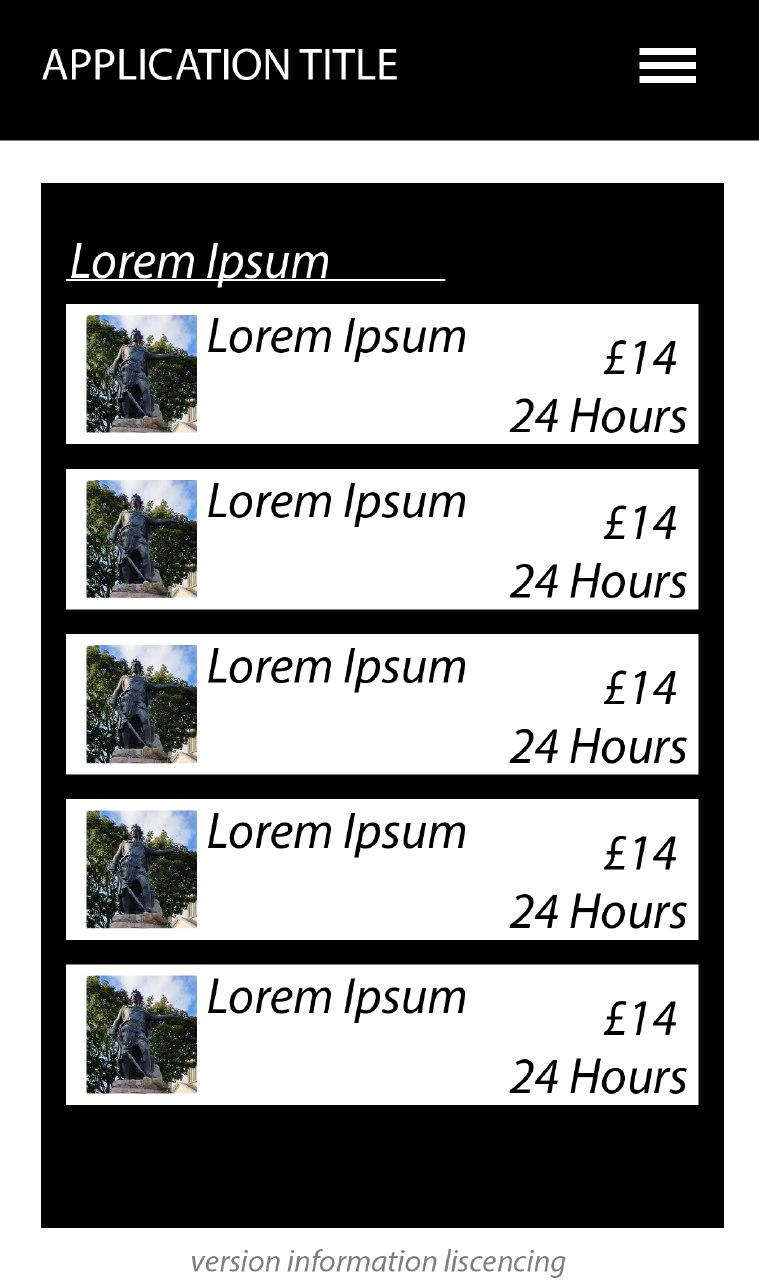
\includegraphics[width=0.5\linewidth]{images/screen1.jpg}} \\
		\hline
		Background & Standard phone background \\
		\hline
		Colour Scehemes Used & Default to black and white but would import from the system theme so users feel immersed \\
		\hline
		Text Attributes & Again, follows system theme (usually a sans-serif font). \\
		\hline
		Audio Files & N/A \\
		\hline
		Video Files & N/A \\
		\hline
		Stills Files & N/A \\
		\hline
		Animations / Movie Clips & N/A \\
		\hline
		\multicolumn{2}{c}{Interface Components (buttons, widgets)} \\
		\hline
		\multicolumn{2}{p{14cm}}{ This page shows a list of "card"-esque locations that match the search term provided by the user on the main page. Above them is the search box that the user can see their current search and make an edit to it.  } \\
		\hline
	\end{tabular}

\hspace{-1cm}
	\centering
	\begin{tabular}{p{4cm}p{10cm}}
		\hline
		Title & tourism app \\
		\hline
		Date & 16th April 2019 \\
		\hline
		Scene & 3 of 4 \\
		\hline
		Description & The selected page \\
		\hline
		Links From Scenes & Scene 1, Scene 2 \\
		\hline
		Links To Scenes & Scene 1, Scene 2 \\
		\hline
		\multicolumn{2}{c}{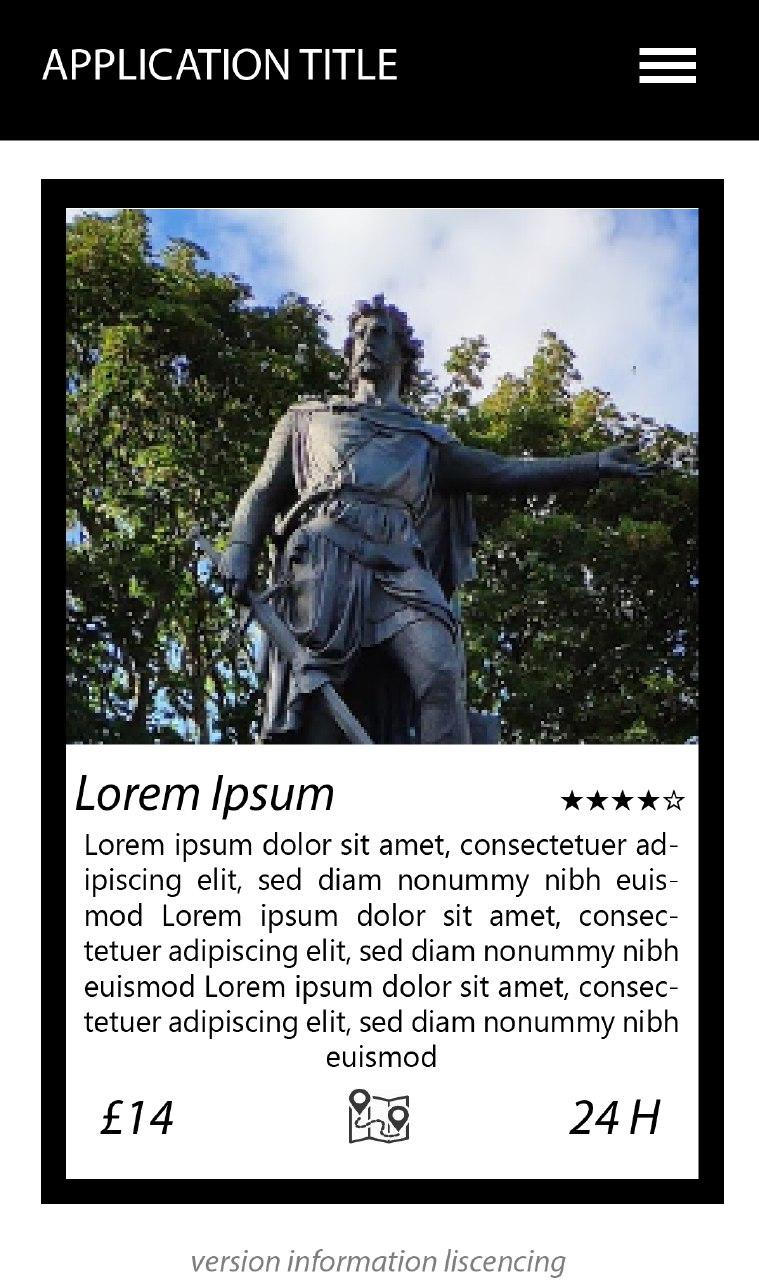
\includegraphics[width=0.5\linewidth]{images/screen2.jpg}} \\
		\hline
		Background & Solid white background on black to highlight the "card design" \\
		\hline
		Colour Scehemes Used & Default to black and white but would import from the system theme so users feel immersed \\
		\hline
		Text Attributes & Again, follows system theme (usually a sans-serif font). \\
		\hline
		Audio Files & N/A \\
		\hline
		Video Files & N/A \\
		\hline
		Stills Files & Header Image for the Location \\
		\hline
		Animations / Movie Clips & N/A \\
		\hline
		\multicolumn{2}{c}{Interface Components (buttons, widgets)} \\
		\hline
		\multicolumn{2}{p{14cm}}{This page contains all of the relevant information pertaining to the attraction. The main content is the image of the location selected by either votes of users or by the maintainers of the attraction. Following this is the Title and the rating on the same line. The rating is powered by user feedback. Next is the description of the attraction of the site which again is chosen by the maintainers. Finally on at the bottom is the price of the venue, a link to get directions to the site and the opening hours.} \\
		\hline
	\end{tabular}

\subsection{Design 2}
\hspace{-1cm}
	\begin{tabular}{p{4cm}p{10cm}}
		\hline
		Title & tourism app \\
		\hline
		Date & 16th April 2019 \\
		\hline
		Scene & 1 of 3 \\
		\hline
		Description & This is the second landing page \\
		\hline
		Links From Scenes & N/A \\
		\hline
		Links To Scenes & Scene 2 \\
		\hline
		\multicolumn{2}{c}{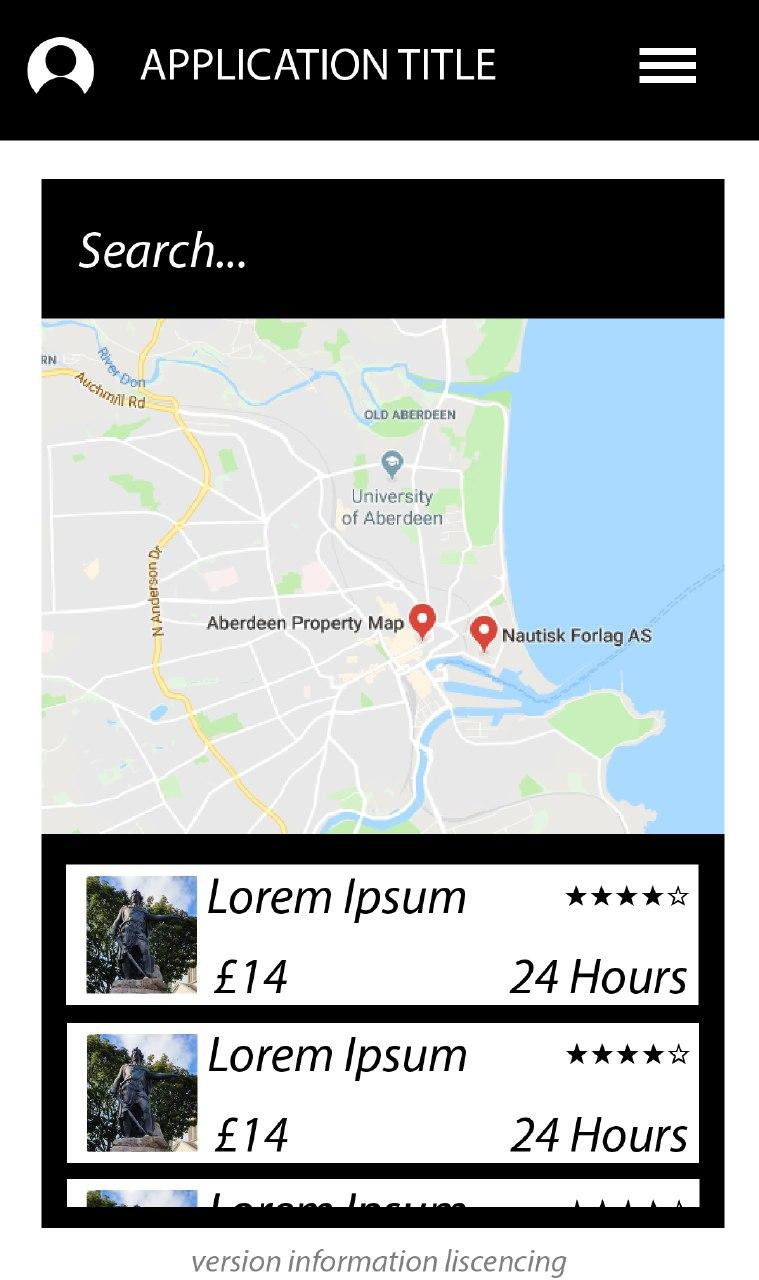
\includegraphics[width=0.5\linewidth]{images/screen0-1.jpg}} \\
		\hline
		Background & Standard phone background \\
		\hline
		Colour Scehemes Used & Default to black and white but would import from the system theme so users feel immersed \\
		\hline
		Text Attributes & Again, follows system theme (usually a sans-serif font). \\
		\hline
		Audio Files & N/A \\
		\hline
		Video Files & N/A \\
		\hline
		Stills Files & N/A \\
		\hline
		Animations / Movie Clips & N/A \\
		\hline
		\multicolumn{2}{c}{Interface Components (buttons, widgets)} \\
		\hline
		\multicolumn{2}{p{14cm}}{The primary screen of the app shows the hamburger menu in the top right of the screen, with the map of the local area in the centre. Above this lies the search box where a user can search for a particular location if they know the name. In addition, the top locations in the area that the user can tap on to get more information. This page has a similar design to the previous however with the profile settings page added in. } \\
		\hline
	\end{tabular}

\hspace{-1cm}
	\begin{tabular}{p{4cm}p{10cm}}
		\hline
		Title & tourism app \\
		\hline
		Date & 16th April 2019 \\
		\hline
		Scene & 2 of 3 \\
		\hline
		Description & The search page of the application \\
		\hline
		Links From Scenes & Scene 1, Scene 3 \\
		\hline
		Links To Scenes & Scene 3 \\
		\hline
		\multicolumn{2}{c}{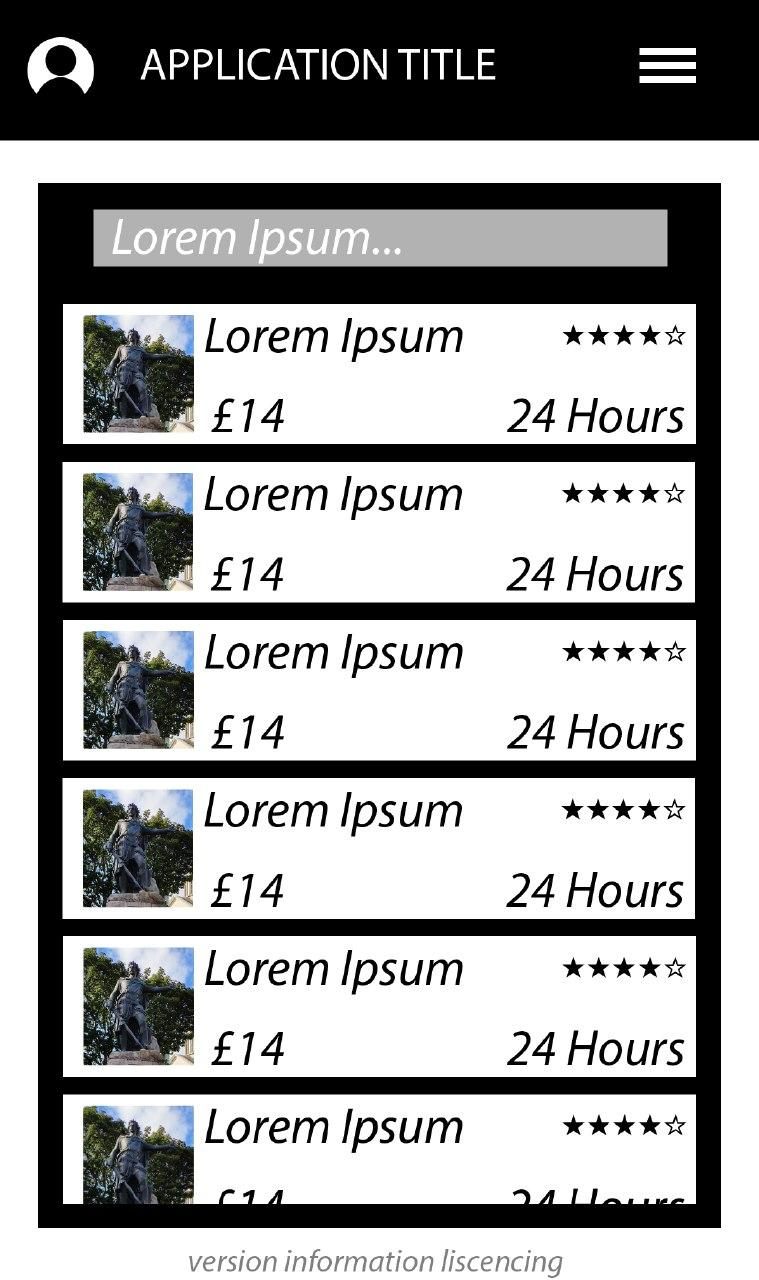
\includegraphics[width=0.5\linewidth]{images/screen1-1.jpg}} \\
		\hline
		Background & Standard phone background \\
		\hline
		Colour Scehemes Used & Default to black and white but would import from the system theme so users feel immersed \\
		\hline
		Text Attributes & Again, follows system theme (usually a sans-serif font). \\
		\hline
		Audio Files & N/A \\
		\hline
		Video Files & N/A \\
		\hline
		Stills Files & Minature pictures included from the primary page photo. \\
		\hline
		Animations / Movie Clips & N/A \\
		\hline
		\multicolumn{2}{c}{Interface Components (buttons, widgets)} \\
		\hline
		\multicolumn{2}{p{14cm}}{ This page shows a list of "card"-esque locations that match the search term provided by the user on the main page. Above them is the search box that the user can see their current search and make an edit to it. In this design the addition of the the rating for each result has been added so that the user can see which is the most highly rated. In addition is the addition of a slight hinting behind the search text to enhance readability and draw the users eye to the search box. } \\
		\hline
	\end{tabular}

\hspace{-1cm}
	\begin{tabular}{p{4cm}p{10cm}}
		\hline
		Title & tourism app \\
		\hline
		Date & 16th April 2019 \\
		\hline
		Scene & 3 of 3 \\
		\hline
		Description & The selected page \\
		\hline
		Links From Scenes & Scene 1, Scene 2 \\
		\hline
		Links To Scenes & Scene 1, Scene 2 \\
		\hline
		\multicolumn{2}{c}{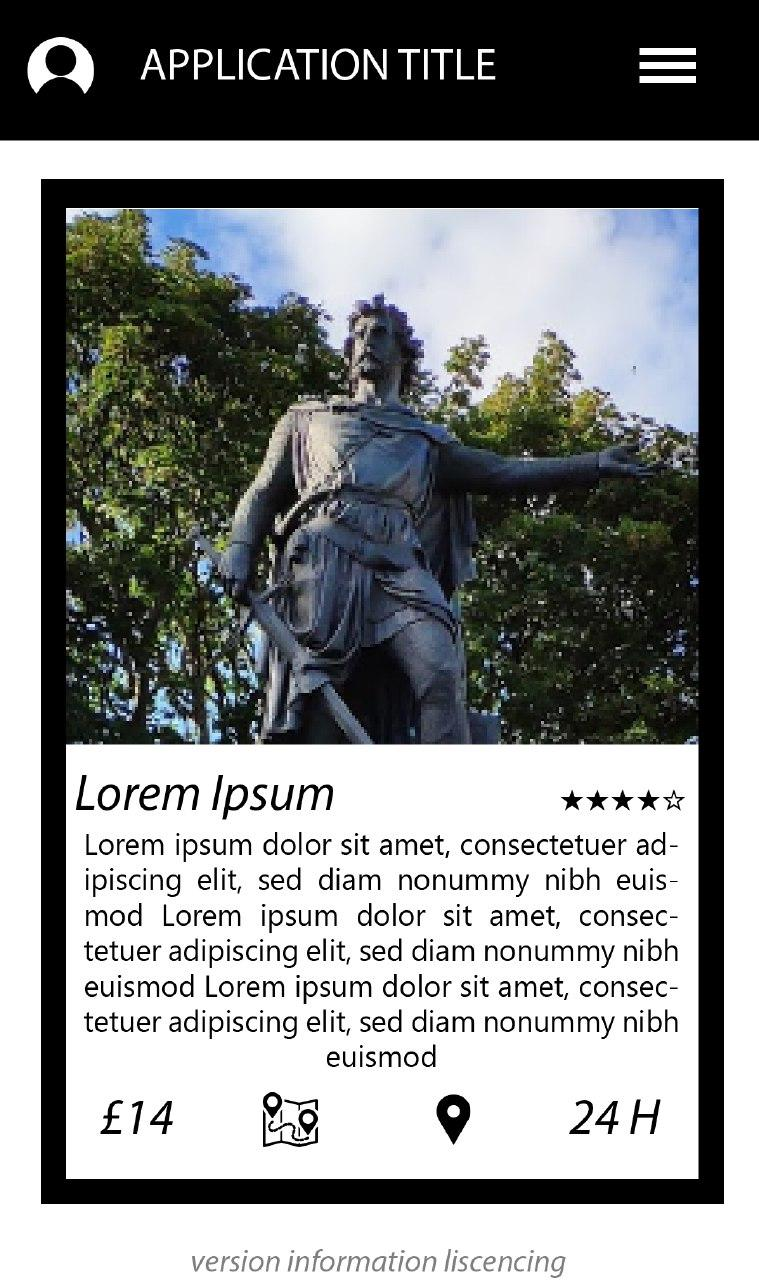
\includegraphics[width=0.5\linewidth]{images/screen2-1.jpg}} \\
		\hline
		Background & Solid white background on black to highlight the "card design" \\
		\hline
		Colour Scehemes Used & Default to black and white but would import from the system theme so users feel immersed \\
		\hline
		Text Attributes & Again, follows system theme (usually a sans-serif font). \\
		\hline
		Audio Files & N/A \\
		\hline
		Video Files & N/A \\
		\hline
		Stills Files & Images provided by the page take up the initil screen in the form of a carousel of images taken or approved by the venue. \\
		\hline
		Animations / Movie Clips & N/A \\
		\hline
		\multicolumn{2}{c}{Interface Components (buttons, widgets)} \\
		\hline
		\multicolumn{2}{p{14cm}}{This page contains all of the relevant information pertaining to the attraction. The main content is the image of the location selected by either votes of users or by the maintainers of the attraction. Following this is the Title and the rating on the same line. The rating is powered by user feedback. Next is the description of the attraction of the site which again is chosen by the maintainers. Finally on at the bottom is the price of the venue, a link to get directions to the site and the opening hours. This page only sees the addition of a "in the area" as requested by the initial round of user questioning, which was a highly requested feature and the "24 Hour" being shurk to make the UI feel more centred. } \\
		\hline
	\end{tabular}

\section{CogTool}
To determine if the additions to design one made in design two negatively or positively affected the use of the application to perform a given task, CogTool was employed.
The previously shown pages were imported as frames and links drawn over to simulate the clickable areas.
Three tasks were chosen in order to give a good overview of the uses of the app and "Think" times were added were appropriate to simulate the use case of a first time user.
These three tasks were carried on on both designs with the same delays applied where appropriate and both designs began in the same place, the homepage.
\begin{table}[H]
\hspace{-0.5cm}
\begin{tabular}{lcc}
\hline
Tasks"&"Design 1"&"Design 2" \\
Search map for a location, select then read desc"&"36.8"&"36.7" \\
Choose top result"&"3.6"&"3.6" \\
Use search to find a destination then find Directions"&"8.2"&"6.8" \\
\hline
\end{tabular}
\end{table}

\begin{table}[H]
\hspace{-2.5cm}
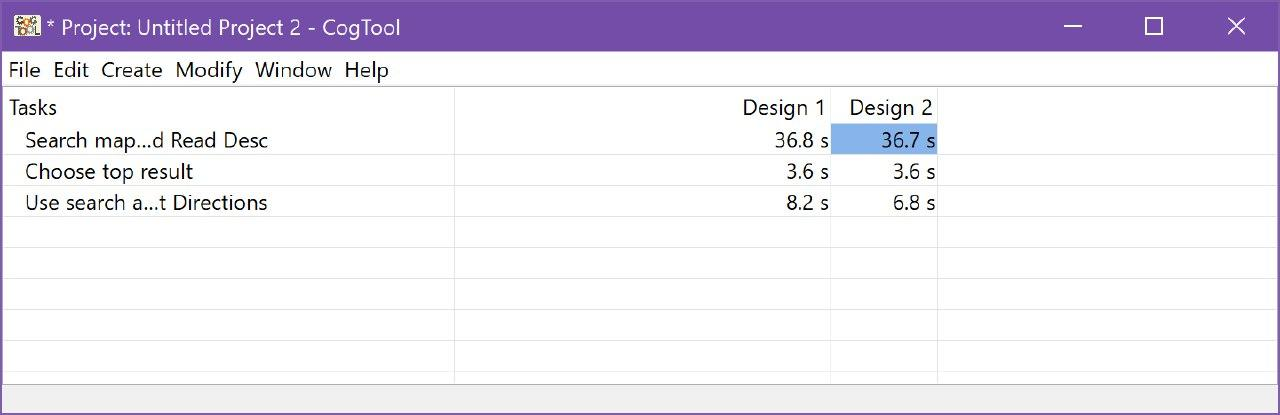
\includegraphics{images/cogtoolresults.jpg}
	\caption{Frame layout for Design 1}
\end{table}
\begin{table}[H]
\hspace{-2.5cm}
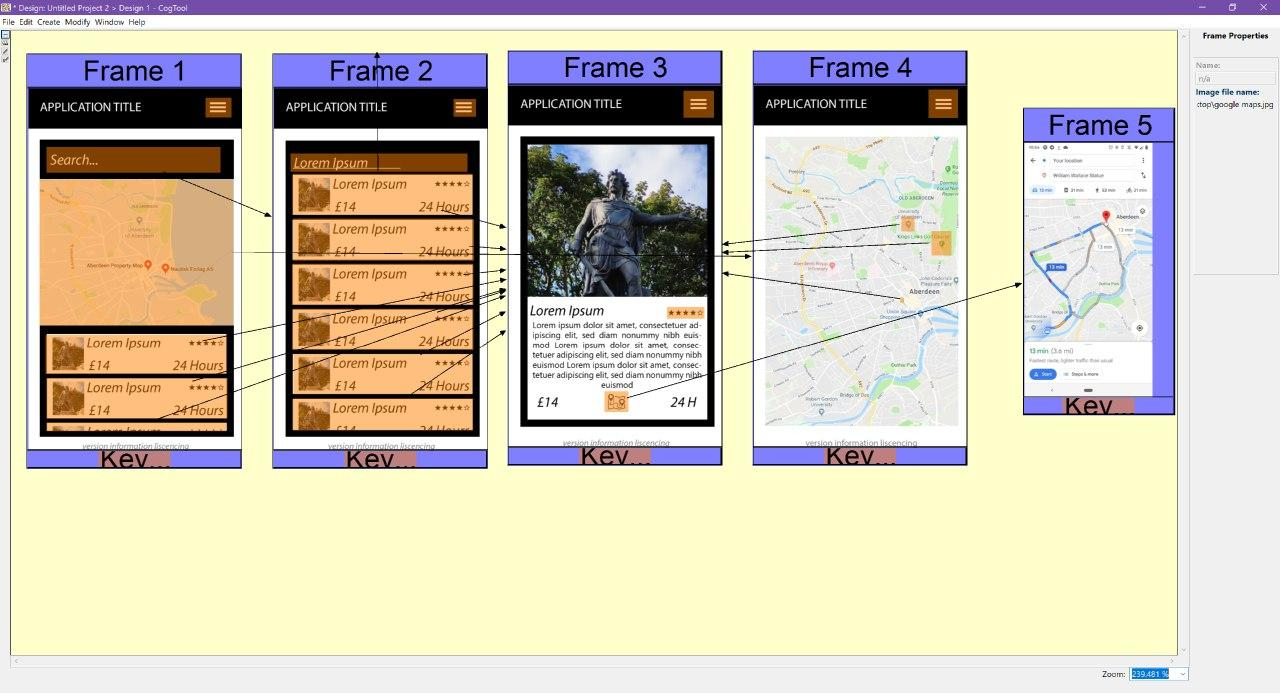
\includegraphics{images/cogtoolframes.jpg}
	\caption{Frame layout for Design 1}
\end{table}

\subsection{Task 1}
Unsurprisingly there was little difference between Design one and Design two which is to be expected as the critical path taken by the user was the same in both designs, only with the addition of some extra buttons that the user has to parse in Design two.
Thankfully though this had no effect on the computational time.
The user is expected, when following this path to arrive on the main page and move into the map screen which is cleary visible on the homescreen.
From here they are allowed a long period of time while the browse the map for a location near to them.
The users then selects the location they have chosen and are taken to the "information" page for that venue.
It is here that the user is also expected to spend an amount of time reading all of the available information, the descriptions varying in length but on average around ~20 seconds.
The ratings on this page allow the user to get an at a glance review of the location and decide whether it is worth continuing reading.
The review section can also be clicked on to expand and reveal the individual reviews, allowing them to be vetted or hints to be shared.
Once the user has decided, the directions button is then clicked which redirects the user to the native maps implementation e.g. Apple Maps, Google Maps or OSM, and the start and destination fields filled for navigation.
The second design merely adds the "local attractions" functionality, returning information about on-site dining and local pubs/restaurant
\subsection{Task 2}
Task 2 again saw little difference between the two paths as it is a very simple path.
The user, from the home page, selects one of the top destinations recommended in the list below the map view.
This then takes them to the information page, and we assume that they ignore the description in this walkthrough and divert them straight to the map.
This is a shorter walkthrough to demonstrate the wide range of users that may be interfacing with the application.
\subsection{Task 3}
Finally in Task 3 we see a difference in the times, dropping two seconds in the second design over the first.
In this task the user, again from the homepage, operates the search bar to initiate a search against the available attractions in the area.
This then returns a scrollable list for the user to peruse.
In the initial design this is a rather spartan layout, however in design two the added ratings and the extra hinting on the search bar to ease the visibility of it, lead to a reduction of two seconds in the operation.
The rating system is likely the most influential as it allows the users to very quickly make a judgement on attraction.
\section{User Evaluation}
\section{Final Changes}
\section{Final Conceptual Design}
\section{Evaluation}
\section{Storyboarding}
\subsection{Shared}
\subsubsection{profile}
The profile button in the top left of all of the pages will allow the user to access the profile management section of the UI.
This page includes the ability to sign in/sign out along with register.
If a logged in user taps on the button they will see the options pertaining to their user such as.
\begin{itemize}
	\item View Reviews
	\item View submitted photos
	\item Change name
\end{itemize}
These options allow basic configurations and changes to be made.
It was important following the user responses to avoid a complex and rich user experience as it seems as though the core functionality expected is what has been listed and anything more get in the way of use.
If a user wanted to perform the action of editing a past review, the process would be as follows.
\begin{enumerate}
	\item Open the application
	\item Tap on the profile button
	\item Choose "View Reviews"
	\item Locate the desired review
	\item Select the edit button
	\item Make nesseccary changes
	\item Select the "Save Changes" button
\end{enumerate}
This would give feedback to the user informing them that the edits were successful, or not, and return them to the list of reviews.
\subsubsection{Menu}
The menu provides a "maximum one click" navigation to all the disperate functions of the application, from anywhere within the application.
This allows the user a point of reference incase they become overwhelmed in the menus and just want to perform a single function.
The use of the "hamburger" iconography is a well recognised symbol representing a menu and thus ensures that the maximum number of people are able to understand and utilize its functionality.
The contents of the menu contains the following.
\begin{itemize}
	\item Home
	\item Map
	\item Top Rated
	\item Profile
	\item Reviews (points to users reviews)
	\item Logout
\end{itemize}
If a user wanted to use the menu to navigate to the map to select a new location near to themselves and they were on the user reviews feeds the process of navigating to it is simple, as described below.
\begin{enumerate}
	\item Tap on the menu icon
	\item Find the desired menu option (Map)
	\item Tap on the desired menu option
\end{enumerate}
This then navigates the user to the maps screen, immediately.
\subsubsection{Search}
The search functionality allows the user to search all of the local attractions.
The returned list is then sorted by the top rated areas, and will offer a greyed out option for places that the user has already visited and reviewed.
This has a dual purpose of helping the user keep track of visited locations while providing an incentive to visit more locations to grey out them all.
This functionality is very well understood by all and simply tapping in the search bar activates the system keyboard so entry can begin.
When the user enters the first character the page is silently moved to the search results page and options appear and are filtered as characters are entered.
\subsubsection{Licence & Version}
As with most open source projects require the displaying of their name and trademark (if they have one) on the application itself this is a good way to booth reassure that the application is up to date.
\subsection{Homepage}
The homepage is the main page of the application as it aggregates the three ways to find the attractions.
\begin{itemize}
	\item Search
	\item Map
	\item Top Feed
\end{itemize}
The search bar is at the top to ensure that the user observes it first as it is the most likely destination for a user.
Following this is the map so that a user can see, at a glance if there is anything nearby and if so, what it is.
Lastly is the top feed, this is most likely used by the user when they don't have a specific destination in mind and just want to explore.
A user landing on the page has a number of options as to how to operate with the application as described above, in this instance we will follow a user who wishes to find the top rated attraction that they have not already visited, regardless of distance or price.
\begin{enumerate}
	\item Open the application
	\item Scroll the page down
	\item Find the first non-grey item
	\item Select it by tapping on it
	\item Ensure that it matches criteria by examining the page
	\item Choose directions (if required)
\end{enumerate}
The app would then helpfully open the, as mentioned before, native maps application (Apple, Google, OSM) and enter navigation mode.
The use of the native application ensures a consistency of design for users unfamiliar with the distinction between first and third party apps and allows the leveraging the power of these map applications.
\subsection{Search / List}
This page contains the results obtained when performing a search.
The list
\section{Conclusion}




\end{document}
